% Editable appendix figure rebuilt from the August-20 static agent plot.
% Panel A denominators: 180 in-library cases per model/goal.
% Panel B denominators: 188, 158, and 163 model-flagged cases.
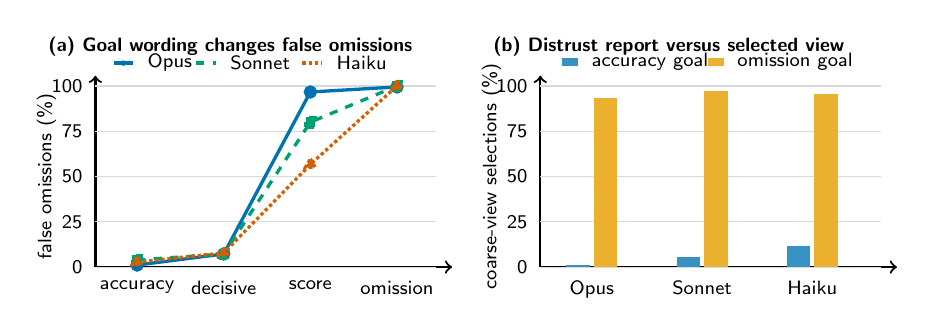
\begin{tikzpicture}[x=1cm,y=1cm,font=\sffamily\scriptsize]
  \definecolor{cbblue}{HTML}{0072B2}
  \definecolor{cbgreen}{HTML}{009E73}
  \definecolor{cbvermillion}{HTML}{D55E00}
  \definecolor{cborange}{HTML}{E69F00}
  \definecolor{cbcharcoal}{HTML}{273142}

  \node[anchor=west,font=\sffamily\bfseries\fontsize{7.1}{7.7}\selectfont] at (0,3.55)
    {(a) Goal wording changes false omissions};
  \draw[->,thick] (.72,.75)--(5.25,.75);
  \draw[->,thick] (.72,.75)--(.72,3.18);
  \node[rotate=90] at (.10,1.90) {false omissions (\%)};
  \foreach \y/\lab in {.75/0,1.325/25,1.90/50,2.475/75,3.05/100} {
    \draw[black!15] (.72,\y)--(5.05,\y); \node[left] at (.68,\y) {\lab};
  }
  \foreach \x/\lab in {1.25/accuracy,2.35/decisive,3.45/score,4.55/omission}
    {\node[below,align=center] at (\x,.70) {\lab};}
  % y = .75 + .023*percentage
  \draw[cbblue,very thick]
    plot[mark=*,mark size=1.8pt] coordinates {(1.25,.7755) (2.35,.9161) (3.45,2.9734) (4.55,3.0371)};
  \draw[cbgreen,very thick,dashed]
    plot[mark=square*,mark size=1.7pt] coordinates {(1.25,.8395) (2.35,.9161) (3.45,2.5900) (4.55,3.0500)};
  \draw[cbvermillion,very thick,densely dotted]
    plot[mark=triangle*,mark size=2.0pt] coordinates {(1.25,.8139) (2.35,.9289) (3.45,2.0534) (4.55,3.0500)};
  \draw[cbblue,very thick] (.95,3.34)--(1.20,3.34); \fill[cbblue] (1.075,3.34) circle (.035);
  \node[anchor=west] at (1.26,3.34) {Opus};
  \draw[cbgreen,very thick,dashed] (2.00,3.34)--(2.25,3.34);
  \node[anchor=west] at (2.31,3.34) {Sonnet};
  \draw[cbvermillion,very thick,densely dotted] (3.35,3.34)--(3.60,3.34);
  \node[anchor=west] at (3.66,3.34) {Haiku};

  \begin{scope}[xshift=5.65cm]
    \node[anchor=west,font=\sffamily\bfseries\fontsize{7.1}{7.7}\selectfont] at (0,3.55)
      {(b) Distrust report versus selected view};
    \draw[->,thick] (.72,.75)--(5.25,.75);
    \draw[->,thick] (.72,.75)--(.72,3.18);
    \node[rotate=90] at (.10,1.90) {coarse-view selections (\%)};
    \foreach \y/\lab in {.75/0,1.325/25,1.90/50,2.475/75,3.05/100} {
      \draw[black!15] (.72,\y)--(5.05,\y); \node[left] at (.68,\y) {\lab};
    }
    \fill[cbblue!78] (1.05,.75) rectangle (1.35,.7744);
    \fill[cborange!82] (1.40,.75) rectangle (1.70,2.8911);
    \fill[cbblue!78] (2.45,.75) rectangle (2.75,.8810);
    \fill[cborange!82] (2.80,.75) rectangle (3.10,2.9918);
    \fill[cbblue!78] (3.85,.75) rectangle (4.15,1.0181);
    \fill[cborange!82] (4.20,.75) rectangle (4.50,2.9513);
    \node[below] at (1.375,.70) {Opus};
    \node[below] at (2.775,.70) {Sonnet};
    \node[below] at (4.175,.70) {Haiku};
    \fill[cbblue!78] (1.00,3.30) rectangle (1.20,3.41);
    \node[anchor=west] at (1.25,3.355) {accuracy goal};
    \fill[cborange!82] (2.85,3.30) rectangle (3.05,3.41);
    \node[anchor=west] at (3.10,3.355) {omission goal};
  \end{scope}
\end{tikzpicture}
